\documentclass[12pt,liststotoc]{report}
\usepackage[T1]{fontenc}
\usepackage[utf8x]{inputenc}
\usepackage{color}
\usepackage{xcolor}
\usepackage{geometry}
\geometry{a4paper, top=25mm, left=25mm, right=25mm, bottom=25mm, headsep=10mm, footskip=12mm} 
\usepackage{amsfonts}
\usepackage{amsmath}
\usepackage[ngerman]{babel}
\usepackage{graphicx}
\usepackage{booktabs}
\usepackage{tabularx}
\usepackage{array}
\usepackage{textcomp}
\usepackage{amssymb}
\usepackage{amstext}
\usepackage{subfigure}
\usepackage{amsfonts}
\usepackage{mathrsfs}
\usepackage{csquotes}
\usepackage{nicefrac}
\usepackage{multirow}
\usepackage{color}
\usepackage{bigstrut}
\usepackage[version=4]{mhchem}
\usepackage{textcomp} 
\usepackage{nicefrac}
\usepackage{lmodern}
\usepackage{pdflscape}
\usepackage{pdfpages}
\usepackage{here} 
\newcommand{\rtab}{\raggedleft\arraybackslash}

\usepackage{hyperref}
\usepackage{fancyref}
\usepackage{todonotes}
\usepackage{bigints}
\usepackage{amsmath}
\usepackage{amssymb}
\usepackage{amstext}
\usepackage{amsfonts}
\usepackage{mathrsfs}
\usepackage[version-1-compatibility]{siunitx}
\usepackage{caption}
\captionsetup{format=plain,justification=centerlast}

%\usepackage[backend=biber,style=alphabetic,sorting=ynt]{biblatex}
%\addbibresource{Quelle_CRT_2.bib} 
 



\usepackage{ngerman}
\setlength{\parindent}{0em}	
\setlength{\parskip}{1.5ex plus0.5ex minus0.5ex}

\usepackage{chemformula}

\captionsetup[table]{skip=5pt}

%\usepackage{tikz}
%\usetikzlibrary{tikzmark}

%\newcommand\zeilestreichen[3][]{%
 % \tikz[remember picture,overlay]\draw[thick,#1]([yshift=0.8ex]pic cs:#2)--([yshift=0.8ex]pic cs:#3);}

\usepackage{soul}

\begin{document}
\setcounter{secnumdepth}{5}
\setcounter{tocdepth}{5}

\begin{titlepage}
	\centering
	
\includegraphics[width=0.5\textwidth]{Graphics/TU_Graz.pdf}\par\vspace{1cm}
	
	{\scshape\LARGE Reaktionstechnik II LU  \par}
	\vspace{1cm}
	{\scshape\Large LU 667.212\par}
	{\scshape \large SS 2018\par}
	\vspace{0.5cm}
	{\huge\bfseries Heterogene Katalyse \par}
	\vspace{0.5cm}

	{\LARGE \itshape Ashok Andermann\par}
	{\large 11729115\par}\vspace{0.5cm}
	%\vspace{0,2cm}	
	
	{\LARGE \itshape Kilian Fleisch\par}
	{\large 11744809\par}\vspace{0.5cm}
	%\vspace{0,2cm}
	
		
	{\LARGE \itshape Jakob Geistlinger\par}
	{\large 01131349\par}\vspace{0.5cm}
	%\vspace{0,2cm}
	
	{\LARGE \itshape Felix Lechleitner\par}
	{\large 01316701\par}\vspace{0.5cm}
	%\vspace{0,2cm}

	{\LARGE \itshape Tobias Maier\par}
	{\large 01330853\par}\vspace{0.5cm}
	%\vspace{0,2cm}
	\vfill

% Bottom of the page
	{\large \today\par}
\end{titlepage}


\pagenumbering{Roman}

\chapter*{Kurzfassung}


In dieser Arbeit wird die Kinetik einer Veresterungsreaktion in einem Rohrreaktor mit einer Länge von 550\,mm und einem Durchmesser von 6\,mm bei 60\,°C untersucht. Die Veresterung von Essigsäure (HAc) und Ethanol (EtOH) zu Ethylacetat (EtAc) und Wasser ist eine reversible Reaktionen mit hoher Aktivierungsenergie, deshalb hat diese Reaktion eine langsame Reaktionsrate. Aus diesem Grund wird die Reaktionen meist katalytisch durchgeführt. Der Katalysator hat die Eigenschaft die Kinetik zu beschleunigen, was besonders für industrielle Zwecke wichtig ist. Als Katalysator wird  $\text{Amberlyst}^\text{\textregistered}$15 verwendet.
\\
\\
Es werden bei vier verschiedenen hydraulischen Verweilzeiten Proben am Reaktorausgang entnommen und mittels Autotitrator die Säurekonzentration ermittelt, wodurch im weiteren Verlauf der Umsatz an Essigsäure kalkuliert werden kann. Dieser Datensatz dient als Grundlage für die Ermittlung der Reaktionsrate und des Zeitgesetzes, wobei die Differentialmethode und Integralmethode am Integralreaktor für hohe Umsätze als Auswertungsmethoden gewählt wird. Vor diesem Schritt wird die Reaktion in ihrer Ordnung beschrieben, wobei aus der Literatur eine reversible Reaktion zweiter Ordnung entnommen wird. 
\\
\\
Bei Auswertung der Kalkulation werden große Abweichungen festgestellt, die jedoch auf experimentelle Fehler wie das Verdampfen der Reaktionsflüssigkeiten nach der Probenahme und der ungenügenden Kühlung zum Inhibieren der Reaktion zurückzuführen sind. Als weitere relevante Fehlerquelle wird die Rundung der Einstellung der Schlauchquetschpumpen festgestellt. Es ist zudem ersichtlich, dass die Integralmethode generell genauere Ergebnisse liefert als die Differentialmethode, da diese auf einem grafischen Verfahren basiert. Allgemein wird der maximale Umsatz bei der größten Verweilzeit von 15\,min mit 57,21\,\%  und der geringste Umsatz bei 2,5\,min Verweilzeit mit 29,07\,\% festgestellt. Die Reaktionsrate variiert aus der Integralmethode zwischen 0,0018 und 0,00029\,mol$\cdot$ g$^{-1} \cdot$ min$^{-1}$ und der Differentialmethode zwischen 0,00167 und 0,00056\,mol$\cdot$ g$^{-1} \cdot$ min$^{-1}$. In einem letzten Schritt wird die ermittelte Kinetik mit der Literatur verglichen, wobei nur qualitative Vergleiche angestellt werden können, da sich bei den gefundenen Literaturquellen zum Beispiel der Aufbau des Versuches oder die Art des Katalysators voneinander unterscheidet. Dennoch ergeben sich Werte in der gleichen Größenordnung. 


\tableofcontents
\newpage
\pagenumbering{arabic}
\chapter{Einleitung \& Aufgabenstellung}

Katalysatoren werden in der chemischen Industrie dazu verwendet, um die Kinetik einer Reaktion zu verändern. Der Katalysator selbst wird dabei weder verbraucht, noch verschiebt er das Gleichgewicht der Reaktion. Durch das Herabsetzen der Aktivierungsenergie $E_A$ läuft die Reaktion schneller ab. Dadurch lassen sich Reaktionen in kürzester Zeit durchführen, welche unter normalen Bedinungen (ohne Kat.) sehr langsam ablaufen. Dies stellt oft die Kostengünstigere Lösung dar, als die Temperatur zu erhöhen oder den Druck zu verändern. Der Mechanismus der heterogenen Katalyse (Kat. und reagierende Stoffe in verschiedenen Phasen) lässt sich in sieben verschiedene Schritte unterteilen \cite{Skript_2018}:

\begin{enumerate}
    \item Konvektiver Transport der Reaktanden an die Oberfläche des Katalysators
    \item Diffusion der Reaktanden in die Poren des Katalysators (aktive Oberfläche)
    \item Adsorption auf die aktive Oberfläche
    \item eigentliche Reaktion
    \item Desorption der reagierten Produkte
    \item Diffusion aus den Poren hinaus
    \item Konvektiver Transport von der Oberfläche des Katalysators in den Bulk
\end{enumerate}

Ziel dieser Laborübung ist es das Zeitgesetz einer katalytischen Veresterungsreaktion zu bestimmen. Die Reaktion von Essigsäure (HAc) und Ethanol (EtOH) zu Essigsäureethylester (EtAc) und Wasser wird bei 60 °C in einem Rohrreaktor durchgeführt. Folglich ist die katalytische Reaktion dargestellt:

\begin{equation}
CH_3COOH + CH_3CH_2OH \stackrel{H^+}{\rightleftharpoons} CH_3COOCH_2CH_3 + H_2O
\end{equation}

Als Katalysator wird $\text{Amberlyst}^\text{\textregistered}$15 verwendet. Zur Ermittlung des Zeitgesetzes werden zwei unterschiedliche Berechnungsmethoden herangezogen und mit einander verglichen. Zur Bestimmung des Zeitgesetzes wird die Integralmethode, sowie die Differentialmethode verwendet. Die Integralmethode wird meist bei Rohrreaktoren mit hohen Reaktionsumsätzen verwendet, wogegen die Differentialmethode bei komplizierten Zeitgesetzen verwendet wird, da ansonsten ein Integral zu lösen ist, welches nicht immer analytisch durchführbar ist. Abschließend werden die beiden Methoden hinsichtlich der Geschwindigkeitskonstante und der Reaktionsrate verglichen und mit Werten aus der Literatur gegenübergestellt.

\chapter{Versuchsaufbau}

Für den Versuch wird der in Abbildung \ref{Prozessfliessbild} und \ref{Versuchsaufbau} dargestellte Aufbau verwendet. Der Reaktor, welcher als Strömungsrohr aufgewickelt ist, ist mit 10\;g des Katalysators gefüllt. Für den Versuch werden 99\,\%-ige Essigsäure (1\,\% deionisiertes Wasser) und 100\;\%-iges Ethanol verwendet. Für die weiteren Berechnungen werden zur Vereinfachung jeweils 100\,\% verwendet.

\begin{figure}[H]
\centering
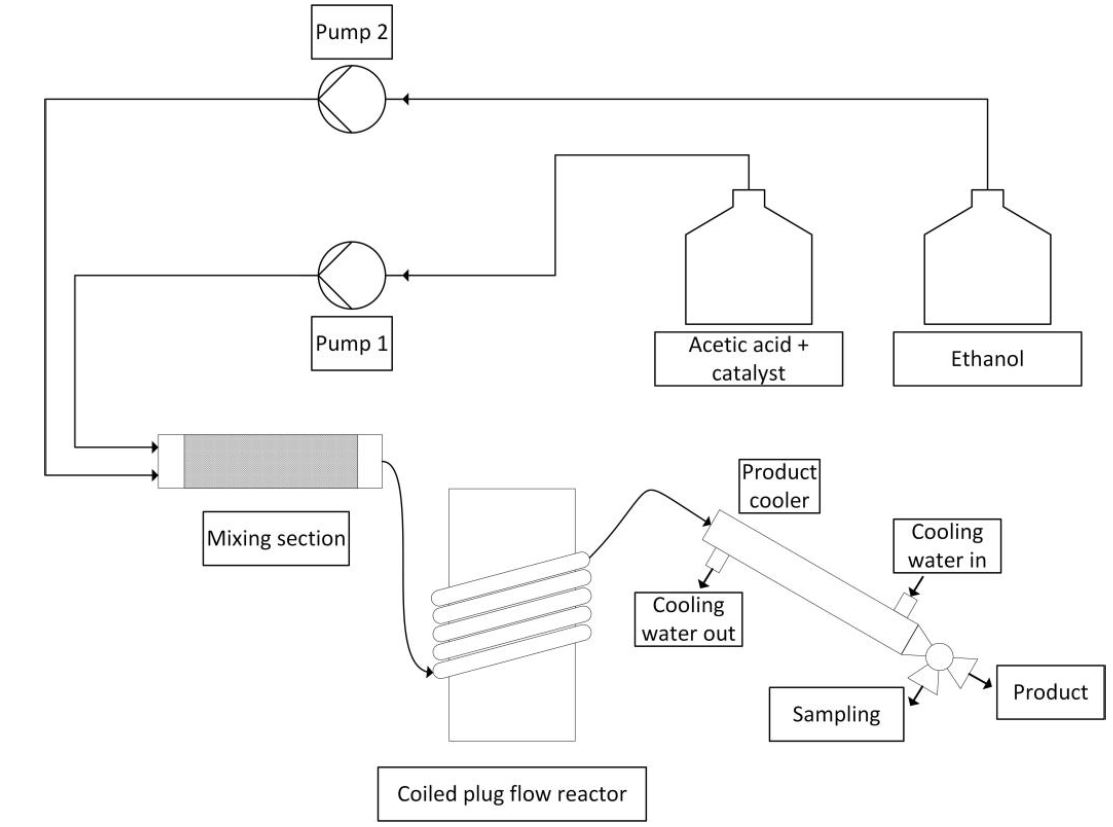
\includegraphics[width=0.8\textwidth]{Graphics/Prozessfliessbild.png} 
\caption[Prozessfließbild des Versuchs]{Prozessfließbild des Versuchs \cite{Labor_Skript2018}}
\label{Prozessfliessbild}
\end{figure}
\noindent

\begin{figure}[H]
\centering
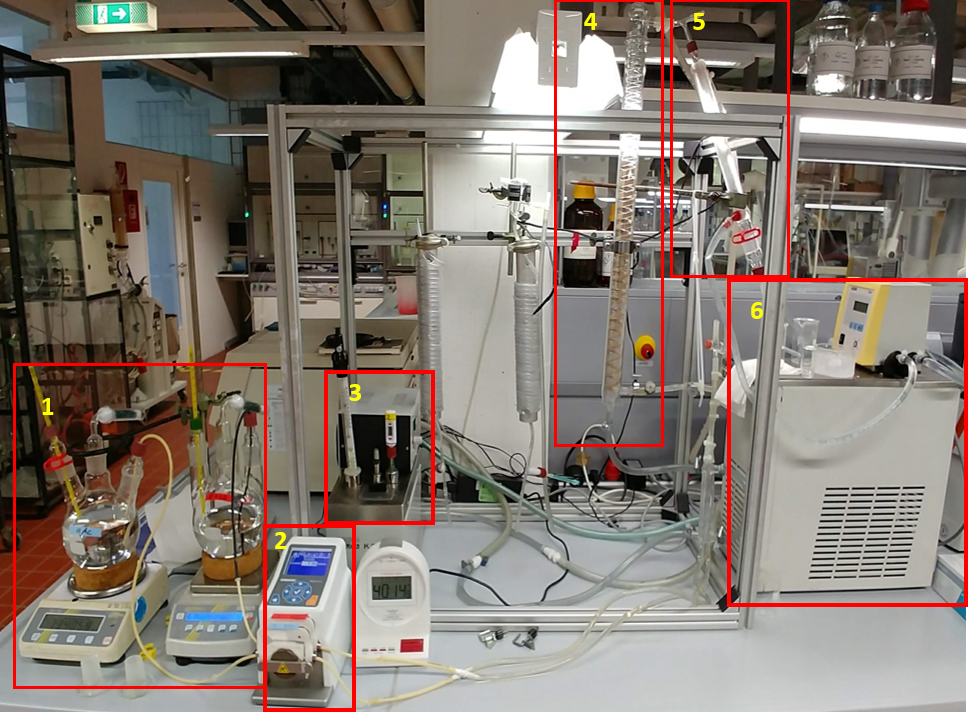
\includegraphics[width=0.8\textwidth]{Graphics/Versuchsaufbau_Veresterung.PNG} 
\caption[Realer Versuchsaufbau vor Ort im Labor]{Realer Versuchsaufbau vor Ort im Labor | 1. Behälter HAc (links) $\&$ EtOH (rechts), 2. Schlauchquetschpumpe, 3. Thermostat, 4. Rohrreaktor $\&$ Mischer (für HAc- und EtOH-Feed) inklusive Raschigringe, 5. Kühler um Reaktion zu unterdrücken, 6. Cryostat des Kühlers}
\label{Versuchsaufbau}
\end{figure}
\noindent

Der Mischer befindet sich vor dem Eingang in den Reaktor und ist explizit in Abbildung \ref{Mischer} dargestellt. Eine Vermischung findet durch die durch Füllkörper verursachten Verwirbelungen und Turbulenzen statt da die Flüssigphasen in intensiven Kontakt miteinander gebracht werden. 

\begin{figure}[H]
\centering
\includegraphics[width=0.8\textwidth]{Graphics/Mischer.png} 
\caption{Mischer mit Raschigringen}
\label{Mischer}
\end{figure}
\noindent

Für die Analyse wird ein automatischer Basentitrator verwendet. Dieser ist in Abbildung \ref{Basentitrator} dargestellt. Die Titration wird mit einmolarer Kalilauge (KOH) durchgeführt. Durch eine auf einem PC installierte Software (Titroline) werden die Messdaten der Titration gesammelt und ausgewertet.

\begin{figure}[H]
\centering
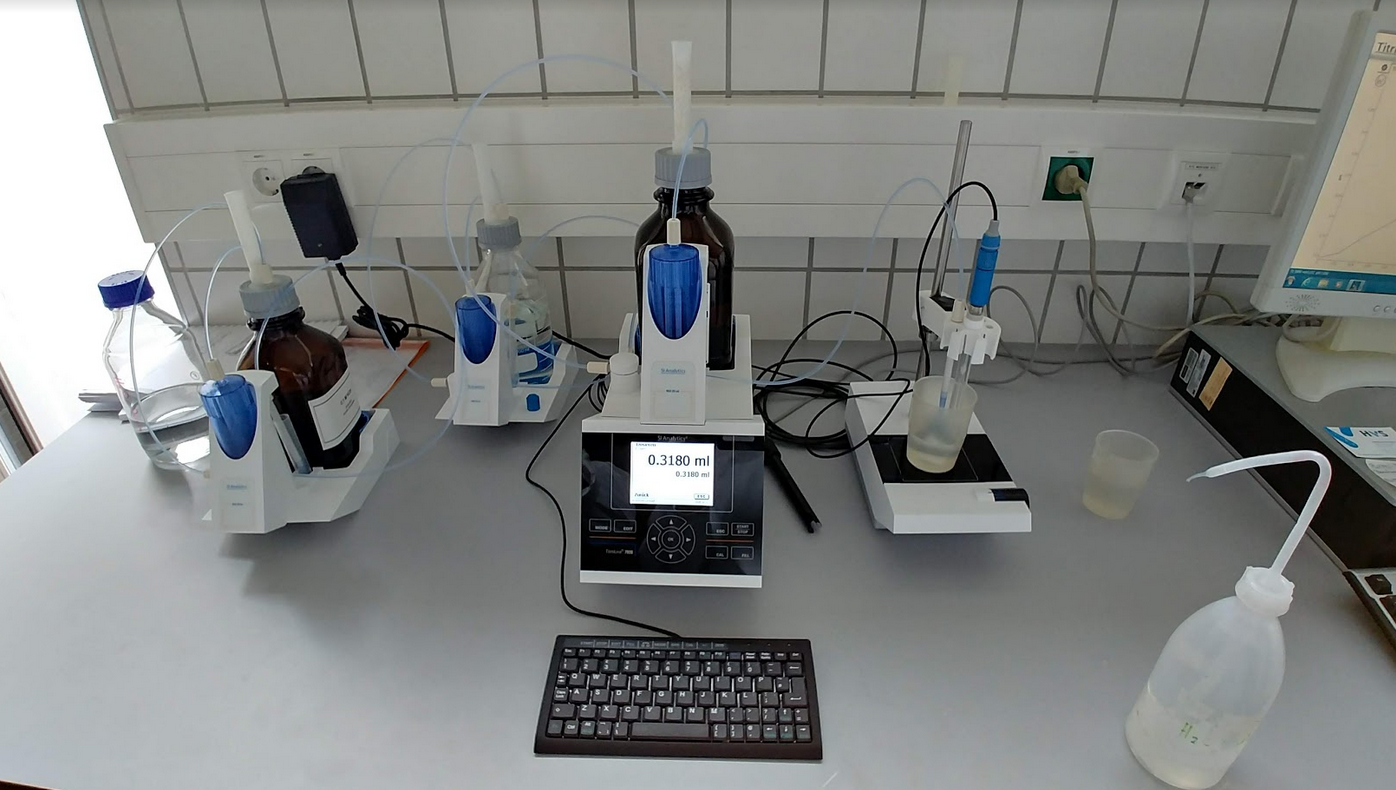
\includegraphics[width=0.8\textwidth]{Graphics/Auto-Basentitrator.PNG} 
\caption[Basentitrator mit vorgelegter Kalilauge]{Basentitrator mit vorgelegter Kalilauge (KOH)}
\label{Basentitrator}
\end{figure}
\noindent


\chapter{Durchführung}

Vor Beginn der Versuche werden die Vorlagen der Essigsäure und Ethanol mittels Heizpilz auf 60\,$\text{°C}$ erwärmt um die vom Vorwärmer zu überwindende Temperaturdifferenz zu minimieren. Zu erwähnen gilt, dass dieser Vorgang beim zweiten Versuch ($\tau = 10\,\min$) nicht gemacht wurde. Dies wurde beim Versuchstag von den Betreuern als nicht relevant eingestuft. 
\\
\\
Vor der eigentlichen Durchführung der Versuche werden die verschiedenen Einstellungen für die benötigen Durchflüsse berechnet. Aus den bereitgestellten Pumpenkalibrationen mit folgenden Gleichungen kann bei bekanntem Massenstrom in $\text{g}\cdot \text{min}^{-1}$ die benötigte Anzahl an Umdrehungen pro Minute kalkuliert werden.

\begin{equation}
\label{PumpeHAc}
    y_{HAc} = x \cdot 0,1426
\end{equation}

\begin{equation}
\label{PumpeEtOH}
     y_{EtOH} = x \cdot 0,1238
\end{equation}


\noindent
Zu Beginn wird ein Molverhältnis  von 2:1 (EtOH : HAc) festgelegt. Um verschiedene Umsätze im experimentellen Verlauf zu erhalten wird die Reaktion bei vier verschiedenen hydraulischen Verweilzeiten durchgeführt. Die molaren Massen von Ethanol und Essigsäure werden aus der NIST Datenbank bezogen  \cite{Ethanol,Essigsaure} und die Dichten mit einem Dichtemessgerät bei 20\,°C ermittelt (Vergleiche \cite{Dichtemessung_Vergleich}). Das Reaktorvolumen wird mit $V_{Reaktor} = 40$\,ml festgelegt, wobei der Rohrreaktor einen Innendurchmesser von $d_{i}$ = 6\,mm und eine Rohrlänge $L_{Rohr}$ = 550\,mm hat und bei den 40\,ml bereits die Volumensverringerung durch Katalysatorpartikel berücksichtigt ist. Somit können die benötigten Informationen in Tabelle \ref{tab:Verweilzeiten} zusammengefasst werden.

\begin{table}[H]
	\caption{Verweilzeiten und Parameter für die Durchflussberechnung}
	\centering
	\begin{tabular}{cc|cccc}
		\toprule 
		Versuchs-Nr. & Verweilzeit $\tau$ in s & $M_{EtOH}$ \cite{Ethanol} & $M_{HAc}$ \cite{Essigsaure}  & $\rho_{EtOH}$  & $\rho_{HAc}$ \\
		&in s&\multicolumn{2}{c}{in $\frac{\text{g}}{\text{mol}}$}&\multicolumn{2}{c}{in $\frac{\text{kg}}{\text{m}^3}$} \\
		\midrule
		1 & 900 & \multirow{4}{*}{60,05} &  \multirow{4}{*}{46,07} & \multirow{4}{*}{789} & \multirow{4}{*}{1050}\\
		2 & 600 \\
		3 & 300 \\
		4 & 150 \\
		\bottomrule
	\end{tabular}
	\label{tab:Verweilzeiten}
\end{table}
\noindent
Im nächsten Schritt kann mit den gesammelten bzw. definierten Daten der gesamte Volumenstrom berechnet werden.

\begin{equation}
    \dot{V}_{ges} = \frac{V_{reaktor}}{\tau}
\end{equation}
\\
\noindent
Mit den bekannten Definitionen der molaren Masse $M = m/n$ und der Dichte $\rho = m/V$ und dem Molverhältnis von 2:1 an Ethanol zu Essigsäure kann der gesamte Stoffstrom $F_{ges}$ bei Umrechnung des Molverhältnisses in ein Volumenverhältnis wie folgt dargestellt werden.

\begin{equation}
 F_{ges} = \frac{\dot{V}_{ges}}{\frac{1}{3} \cdot \frac{M_{HAc}}{\rho_{HAc}} + \frac{2}{3} \cdot \frac{M_{EtOH}}{\rho_{EtOH}}}  
\end{equation}
\\
\noindent
Somit ist der Massenstrom an EtOH und HAc bestimmbar.

\begin{align}
    \dot{m}_{HAc} &= \frac{1}{3} \cdot F_{ges} \cdot M_{HAc} \\
    \notag\\
    \dot{m}_{EtOH} &= \frac{2}{3} \cdot F_{ges} \cdot M_{EtOH}
\end{align}
\\
\noindent 

Mit den Gleichungen der Kalibrationsgeraden  (\ref{PumpeHAc}) bzw. (\ref{PumpeEtOH}) werden die Umdrehungen der Schlauchquetschpumpen pro Minute bestimmt.

\begin{equation*}
    RPM_{HAc} = \frac{\dot{m}_{HAc} }{0,1426}
\end{equation*}
\noindent
\begin{center}bzw.\end{center}
\begin{equation*}
    RPM_{EtOH} = \frac{\dot{m}_{EtOH}}{0,1238}
\end{equation*}
\\
\noindent
Die erhaltenen Ergebnisse sind in Tabelle \ref{tab:Umdrehungen} zusammengefasst.

\begin{table}[H]
	\caption{Umdrehungen der Pumpe der einzelnen Versuche}
	\centering
	\begin{tabular}{c|cc|cc}
		\toprule 
		\multirow{3}{*}{Versuchs-Nr}&\multicolumn{2}{ c| }{berechnete Umdrehungen}&\multicolumn{2}{ c }{eingestellte Umdrehungen}\\
		& HAc & EtOH & HAc & EtOH  \\
		&\multicolumn{2}{ c| }{in $\frac{\text{U}}{\text{min}}$}&\multicolumn{2}{ c }{in $\frac{\text{U}}{\text{min}}$}\\ \midrule
		1&4,39&13,19&4&13\\
		2&6,59&19,79&7&20\\
		3&13,18&39,58&13&40\\
		4&26,36&79,15&26&79\\
		\bottomrule
	\end{tabular}
	\label{tab:Umdrehungen}
\end{table}
\noindent
Für jede Versuchsreihe - also jeden Durchfluss - nach Einstellung der jeweiligen Pumpendrehzahl wird bis zum eigentlichen Versuchsstart die 3-fache theoretische Verweilzeit gewartet um einen stationäre Betrieb zu garantieren. Vor und nach dieser Einlaufzeit wird das aktuelle Gewicht der Vorlagegefäße bestimmt um im weiteren Verlauf den genauen Massendurchsatz für die jeweilige Versuchsreihe zu erhalten.

Anschließend werden am Ende des Reaktors die Proben entnommen, welche sogleich in Eiswasser gekühlt werden. Dies dient zum einen der deutlichen Reduktion der Reaktionsgeschwindigkeit und der Unterbindung der Verflüchtigung der Komponenten. Davon werden 0,5 $\text{ml}$ der jeweiligen Probe in ein Titriergefäß pipettiert und die genaue Masse bestimmt. Mittels Autotitrator wird dann der Säuregehalt der Probe bestimmt.
Der  zeitbestimmende Schritt bei der Probenahme ist die Titration, da Totzeiten zwischen der Probenahme und der Titration unbedingt vermieden werden sollen um den Einfluss von weiterer Reaktion und Verflüchtigung zu minimieren.
Zu jedem Durchfluss werden 5 Proben gezogen um die Möglichkeit zu erhalten mögliche Ausreißer zu streichen und dennoch repräsentative Ergebnisse zu erhalten.
Nach Abschluss der Übung werden die Pumpe sowie Kryostat und Thermostat heruntergefahren und sämtliche Chemikalien ordnungsgemäß entsorgt.




\chapter{Ergebnisse $\&$ Interpretation}

\section{Auswertung der Proben und Umsatzberechnung}
\label{auswertungundumsatzberechnung}

Für die Umsatzberechnung müssen die Start- und Endkonzentration der Essigsäure ermittelt werden. Desweiteren wird noch die tatsächliche Verweilzeit und das tatsächliche Verhältnis der Edukte bestimmt.\\
\\
Um die Anfangskonzentration zu ermitteln wird zunächst der Massenstrom aus der Massendifferenz, welche sich über die Einlaufzeit ergibt, berechnet.

\begin{align}
    \dot{m}_{HAc} &= \frac{m_{HAc, 0} - m_{HAc}}{t}\\
    \notag\\
    \dot{m}_{EtOH} &= \frac{m_{EtOH, 0} - m_{EtOH}}{t}
\end{align}

Über die molare Masse wird der Massenstrom in den Molenstrom umgerechnet.

\begin{align}
    F_{HAc,0} = \frac{\dot{m}_{HAc}}{M_{HAc}}\\
    \notag\\
    F_{EtOH,0} = \frac{\dot{m}_{EtOH}}{M_{EtOH}}
\end{align}

Mit den Stoffmengenströmen der beiden Edukte kann das Stoffmengenverhältnis $y$ berechnet werden.

\begin{equation}
    y = \frac{F_{EtOH,0}}{F_{HAc,0}}
\end{equation}

Durch den Bezug des Molenstroms auf den gesamten Massenstrom wird die Konzentration berechnet.

\begin{equation}
    c_{HAc, 0} = \frac{F_{HAc,0}}{\dot{m}_{HAc} + \dot{m}_{EtOH} }
\end{equation}


Die Endkonzentration berechnet sich aus dem Ergebnis der Titration.
%Die benötigte Stoffmenge an KOH entspricht der vorhandenen Stoffmenge HAc in der Probe. Mit dem benötigten Volumen KOH und der Konzentration der verwendeten Kalilauge wird die Stoffmenge Essigsäure berechnet.
Im Rahmen der Probenahme wird die entnommene Probe ins Titriergefäß pipettiert und mit einer Analysewaage abgewogen. Das Volumen an zugegebener Kalilauge zum Erreichen des Äquivalenzpunktes wird mit dem Autotitrator ermittelt und mit der bekannten Neutralisationsreaktion von KOH mit Essigsäure kann durch das stöchiometrische 1:1 Verhältnis die Konzentration an HAc in der Ausgangsprobe berechnet werden. Die Reaktion bildet das Kaliumsalz der Essigsäure, Kaliumacetat ($CH_3COOK$).

\begin{equation}
    \ce{CH_3COOH + KOH \rightarrow CH_3COOK + H2O}
\end{equation}

Daraus ergibt sich, dass:

\begin{equation}
    n_{HAc,1} = V_{KOH} \cdot c_{KOH}
\end{equation}

Die Stoffmenge wird auf die Masse der gezogenen Probe bezogen um die Konzentration zu erhalten.

\begin{equation}
c_{HAc,1} = \frac{n_{HAc,1}}{m_{Probe}}
\end{equation}

Somit kann der Umsatz berechnet werden.

\begin{equation}
    X_{HAc} = \frac{c_{HAc,0} - c_{HAc,1}}{c_{HAc,0}}
\end{equation}

Um die tatsächliche Verweilzeit $\tau_{real}$ zu berechnen werden die Massenströme über die jeweiligen Dichten in Volumenströme umgerechnet, addiert und durch das Reaktorvolumen dividiert.

\begin{align}
    &\dot{V}_{HAc} = \frac{\dot{m}_{HAc}}{\rho_{HAc}}\\
    \notag\\
    &\dot{V}_{EtOH} = \frac{\dot{m}_{EtOH}}{\rho_{EtOH}}\\
    \notag\\
    &\tau_{real} = \frac{V_{Reaktor}}{\dot{V}_{HAc} + \dot{V}_{EtOH}}
\end{align}



%Mit bekannten Verweilzeiten und den Massendifferenzen der EtOH- und HAc-Vorlagebehälter kann der tatsächliche Massenstrom der Edukte und in weiterer Folge der Volumenstrom, Stoffstrom und damit die Konzentration an Essigsäure am Mischpunkt bestimmt werden. Mit der Eingabe der Probemasse welche im Titriergefäß vorhanden ist und dem Ergebnis der Autotitration, dem Volumen an 1\,mol$\cdot$l$^{-1}$ Kalilauge $KOH$, wird die Konzentration an Essigsäure in der Probe ermittelt.
%\\
%\\
%Die Massendifferenzen für die jeweiligen Verweilzeiten $\tau$ sind in den Tabellen \ref{tab:Umsatzzusammenfassung} und \ref{tab:Umsatzzusammenfassung2} zusammengefasst, wobei die Massenströme durch Division der Massendifferenz mit der Verweilzeit erhalten werden können ($\dot{M} = \Delta M / \tau$). In weiterer Folge kann mit der bekannten Dichte in Tabelle \ref{tab:Verweilzeiten} der Volumenstrom durch $\dot{V} = \dot{M}/\rho$ und der gesamte Volumenstrom durch Addition der beiden Komponentenströme kalkuliert werden. 
%\\
%\\
%Diese Schritte werden durchexerziert um die tatsächliche Verweilzeit zu bestimmen, indem das Reaktorvolumen $V_{Reaktor}$ = 40\,ml durch den gesamten Volumenstrom dividiert wird.
%
%\begin{equation}
% \tau_{real} = \frac{V_{Reaktor}}{\dot{V}_{ges}}   
%\end{equation}
%\noindent
%Durch Heranziehen der molaren Massen an EtOH und HAc wird der tatsächliche Stoffstrom mittels $\dot{N} = m_{i} / M_{i}$ berechnet um damit die Konzentration an Essigsäure (Ethanol wird an dieser Stelle nicht benötigt) mit dem Stoffstrom und der gesamten verbrauchten Masse, nicht dem Massenstrom, zu erhalten.
%
%\begin{equation*}
%    c_{HAc,0} = \frac{\dot{N}_{HAc}}{m_{HAc} + m_{EtOH}}
%\end{equation*}
%\noindent
%Im Rahmen der Probenahme wird die entnommene Probe ins Titriergefäß pipettiert und mit einer Analysewaage abgewogen. Das Volumen an zugegebener Kalilauge zum Erreichen des Äquivalenzpunktes wird mit dem Autotitrator ermittelt und mit der bekannten Neutralisationsreaktion von KOH mit Essigsäure kann durch das stöchiometrische 1:1 Verhältnis die Konzentration an HAc in der Ausgangsprobe berechnet werden. Die Reaktion bildet das Kaliumsalz der Essigsäure, Kaliumacetat ($CH_3COOK$).
%
%\begin{equation}
%    \ce{CH_3COOH + KOH \rightarrow CH_3COOK + H2O}
%\end{equation}
%
%\begin{equation*}
%    c_{HAc} = \frac{N_{HAc}}{m_{probe}}
%\end{equation*}
%\noindent
%Es ist dabei auf die Einheiten zu achten (z.B. ml KOH aus Autotitrator in l).
%\\
%\\
%In weiterer Folge kann dann der benötigte Umsatz an Essigsäure über die Anfangs- und Endkonzentration am Reaktoreingang (Index 0) bzw. -ausgang (Index 1) kalkuliert werden.
%
%\begin{equation}
%    X_{HAc} = \frac{c_{HAc,0} - c_{HAc,1}}{c_{HAc,0}}
%\end{equation}
%\noindent
Die berechneten bzw. gemessenen Daten sind für alle vier Verweilzeiten in den Tabellen \ref{tab:Umsatzzusammenfassung} und \ref{tab:Umsatzzusammenfassung2} zusammengefasst.


\begin{landscape}

%% Table generated by Excel2LaTeX from sheet 'Umsatzberechnung (2)'
%\begin{table}[htbp]
%	\centering
%	\caption{Experimentelle und berechnete Daten zur Umsatzbestimmung}
%	\begin{tabular}{ccccccccccccccccc}
%		\toprule
%		$\tau_{soll}$ & $t$ & $M_{HAc}$ & $M_{ETOH}$ & $\dot{m}_{HAc}$ & $\dot{m}_{EtOH}$ & $\dot{V}_{HAc}$ & $\dot{V}_{EtOH}$ & $\dot{V}_{ges}$& $\tau_{real}$  &  $\dot{N}_{HAc,0}$ & $c_{HAc,0}$ & $m_{Probe}$ & $V_{KOH}$  & $\dot{N}_{HAc,1}$ & $c_{HAc,1}$& $X_{HAc}$ \\
%		min & min & g & g & $\frac{\text{g}}{\text{min}}$ &  $\frac{\text{g}}{\text{min}}$ &  $\frac{\text{ml}}{\text{min}}$ & $\frac{\text{ml}}{\text{min}}$ &  $\frac{\text{ml}}{\text{min}}$ & min     & $\frac{\text{mol}}{\text{min}}$ & $\frac{\text{mol}}{\text{g}}$ & g & ml  & $\frac{\text{mol}}{\text{min}}$ & $\frac{\text{mol}}{\text{g}}$ & - \\
%		\midrule
%		\multirow{6}[2]{*}{15 min} & 0.000 & 1433.220 & 1163.050 & -     & -     & -     & -     & -     & -     & -     & -     & -     & -     & -     & -     &  \\
%		& 45.000 & 1403.790 & 1090.010 & 0.654 & 1.623 & 0.623 & 2.057 & 2.680 & 14.925 & 0.014 & 0.006 & 0.424 & 1.368 & 0.001 & 0.003 & 0.483 \\
%		&       &       &       & 0.654 & 1.623 &       &       &       &       & 0.014 & 0.006 & 0.304 & 0.935 & 0.001 & 0.003 & 0.507 \\
%		&       &       &       & 0.654 & 1.623 &       &       &       &       & 0.014 & 0.006 & 0.429 & 1.253 & 0.001 & 0.003 & 0.532 \\
%		&       &       &       & 0.654 & 1.623 &       &       &       &       & 0.014 & 0.006 & 0.412 & 1.098 & 0.001 & 0.003 & 0.572 \\
%		&       &       &       & 0.654 & 1.623 &       &       &       &       & 0.014 & 0.006 & 0.428 & 1.153 & 0.001 & 0.003 & 0.568 \\
%		\midrule
%		\multirow{6}[2]{*}{10 min} & 0.000 & 1385.730 & 1045.340 & -     & -     & -     & -     & -     & -     & -     & -     & -     & -     & -     & -     &  \\
%		& 30.000 & 1351.830 & 971.880 & 1.130 & 2.449 & 1.076 & 3.104 & 4.180 & 9.570 & 0.025 & 0.007 & 0.430 & 1.351 & 0.001 & 0.003 & 0.542 \\
%		&       &       &       & 1.130 & 2.449 &       &       &       &       & 0.025 & 0.007 & 0.412 & 1.362 & 0.001 & 0.003 & 0.518 \\
%		&       &       &       & 1.130 & 2.449 &       &       &       &       & 0.025 & 0.007 & 0.431 & 1.455 & 0.001 & 0.003 & 0.508 \\
%		&       &       &       & 1.130 & 2.449 &       &       &       &       & 0.025 & 0.007 & 0.424 & 1.435 & 0.001 & 0.003 & 0.506 \\
%		&       &       &       & 1.130 & 2.449 &       &       &       &       & 0.025 & 0.007 & 0.433 & 1.461 & 0.001 & 0.003 & 0.508 \\
%		\midrule
%		\multirow{6}[2]{*}{5 min} & 0.000 & 1317.820 & 898.060 & -     & -     & -     & -     & -     & -     & -     & -     & -     & -     & -     & -     &  \\
%		& 15.000 & 1286.970 & 826.740 & 2.057 & 4.755 & 1.959 & 6.026 & 7.985 & 5.009 & 0.045 & 0.007 & 0.427 & 1.785 & 0.002 & 0.004 & 0.362 \\
%		&       &       &       & 2.057 & 4.755 &       &       &       &       & 0.045 & 0.007 & 0.420 & 1.744 & 0.002 & 0.004 & 0.366 \\
%		&       &       &       & 2.057 & 4.755 &       &       &       &       & 0.045 & 0.007 & 0.432 & 1.794 & 0.002 & 0.004 & 0.366 \\
%		&       &       &       & 2.057 & 4.755 &       &       &       &       & 0.045 & 0.007 & 0.426 & 1.568 & 0.002 & 0.004 & 0.438 \\
%		&       &       &       & 2.057 & 4.755 &       &       &       &       & 0.045 & 0.007 & 0.427 & 1.711 & 0.002 & 0.004 & 0.389 \\
%		\midrule
%		\multirow{7}[2]{*}{2,5 min} & 0.000 & 1210.440 & 1129.070 & -     & -     & -     & -     & -     & -     & -     & -     & -     & -     & -     & -     &  \\
%		& 9.000 & 1174.400 & 1047.510 & 4.004 & 9.062 & 3.814 & 11.486 & 15.299 & 2.614 & 0.087 & 0.007 & 0.482 & 1.924 & 0.002 & 0.004 & 0.400 \\
%		&       &       &       & 4.004 & 9.062 &       &       &       &       & 0.087 & 0.007 & 0.333 & 1.571 & 0.002 & 0.005 & 0.291 \\
%		&       &       &       & 4.004 & 9.062 &       &       &       &       & 0.087 & 0.007 & 0.340 & 1.571 & 0.002 & 0.005 & 0.305 \\
%		&       &       &       & 4.004 & 9.062 &       &       &       &       & 0.087 & 0.007 & 0.343 & 1.499 & 0.001 & 0.004 & 0.343 \\
%		&       &       &       & 4.004 & 9.062 &       &       &       &       & 0.087 & 0.007 & 0.386 & 1.658 & 0.002 & 0.004 & 0.355 \\
%		&       &       &       & 4.004 & 9.062 &       &       &       &       & 0.087 & 0.007 & 0.340 & 1.539 & 0.002 & 0.005 & 0.319 \\
%		\bottomrule
%	\end{tabular}%
%	\label{tab:Umsatzzusammenfassung}%
%\end{table}%

% Table generated by Excel2LaTeX from sheet 'Tabelle6'
\begin{table}[htbp]
  \centering
  \caption[Gemessene Daten für alle vier Verweilzeiten]{Gemessene Daten für alle vier Verweilzeiten inklusive deren berechneter Parameter}
    \begin{tabular}{ccccccccccccccc}
    \toprule
    $\tau$ & $t$   & $m_{HAc}$ & $m_{EtOH}$ & $\dot{m}_{HAc}$ & $\dot{m}_{EtOH}$ & $\dot{V}_{HAc}$ & $\dot{V}_{EtOH}$ & $\dot{V}_{ges}$ & $\tau_{real}$ & $F_{HAc}$ & $F_{EtOH}$ & $c_{HAc,0}$ & $c_{EtOH,0}$ & y \\
    min   & min   & g     & g     & $\frac{\text{g}}{\text{min}}$ & $\frac{\text{g}}{\text{min}}$ & $\frac{\text{ml}}{\text{min}}$ & $\frac{\text{ml}}{\text{min}}$ & $\frac{\text{ml}}{\text{min}}$ & min   & $\frac{\text{mol}}{\text{min}}$ & $\frac{\text{mol}}{\text{min}}$ & $\frac{\text{mol}}{\text{g}}$ & $\frac{\text{mol}}{\text{g}}$ & - \\
    \midrule
    \multirow{2}[2]{*}{15 min} & 0     & 1433,22 & 1163,05 & \multirow{2}[2]{*}{0,654} & \multirow{2}[2]{*}{1,623} & \multirow{2}[2]{*}{0,623} & \multirow{2}[2]{*}{2,057} & \multirow{2}[2]{*}{2,680} & \multirow{2}[2]{*}{14,925} & \multirow{2}[2]{*}{0,014} & \multirow{2}[2]{*}{0,027} & \multirow{2}[2]{*}{0,006} & \multirow{2}[2]{*}{0,012} & \multirow{2}[2]{*}{1,904} \\
          & 45    & 1403,79 & 1090,01 &       &       &       &       &       &       &       &       &       &       &  \\
    \midrule
    \multirow{2}[2]{*}{10 min} & 0     & 1385,73 & 1045,34 & \multirow{2}[2]{*}{1,130} & \multirow{2}[2]{*}{2,449} & \multirow{2}[2]{*}{1,076} & \multirow{2}[2]{*}{3,104} & \multirow{2}[2]{*}{4,180} & \multirow{2}[2]{*}{9,570} & \multirow{2}[2]{*}{0,025} & \multirow{2}[2]{*}{0,041} & \multirow{2}[2]{*}{0,007} & \multirow{2}[2]{*}{0,011} & \multirow{2}[2]{*}{1,662} \\
          & 30    & 1351,83 & 971,88 &       &       &       &       &       &       &       &       &       &       &  \\
    \midrule
    \multirow{2}[2]{*}{5 min} & 0     & 1317,82 & 898,06 & \multirow{2}[2]{*}{2,057} & \multirow{2}[2]{*}{4,755} & \multirow{2}[2]{*}{1,959} & \multirow{2}[2]{*}{6,026} & \multirow{2}[2]{*}{7,985} & \multirow{2}[2]{*}{5,009} & \multirow{2}[2]{*}{0,045} & \multirow{2}[2]{*}{0,079} & \multirow{2}[2]{*}{0,007} & \multirow{2}[2]{*}{0,012} & \multirow{2}[2]{*}{1,774} \\
          & 15    & 1286,97 & 826,74 &       &       &       &       &       &       &       &       &       &       &  \\
    \midrule
    \multirow{2}[2]{*}{2,5 min} & 0     & 1210,44 & 1129,07 & \multirow{2}[2]{*}{4,004} & \multirow{2}[2]{*}{9,062} & \multirow{2}[2]{*}{3,814} & \multirow{2}[2]{*}{11,486} & \multirow{2}[2]{*}{15,299} & \multirow{2}[2]{*}{2,614} & \multirow{2}[2]{*}{0,087} & \multirow{2}[2]{*}{0,151} & \multirow{2}[2]{*}{0,007} & \multirow{2}[2]{*}{0,012} & \multirow{2}[2]{*}{1,736} \\
          & 9     & 1174,4 & 1047,51 &       &       &       &       &       &       &       &       &       &       &  \\
    \bottomrule
    \end{tabular}%
  \label{tab:Umsatzzusammenfassung}%
\end{table}%
%\todo{Beschreibung der Tabelle, war letztes Mal ein Streitpunkt}
\newline
Tabelle \ref{tab:Umsatzzusammenfassung} zeigt die gemessen bzw. berechneten Daten der vier Versuche. Lediglich $m_{HAc}$ und $m_{EtOH}$ sind gemessene Werte. Das ist die Masse von Essigsäure und Ethanol in den jeweiligen Vorlagebehältern, welche zum Zeitpunkt Null (Versuchsstart) und am Ende des Versuchs ($t=45$; $t=30$; $t=15$; $t=9\,\text{min}$) bestimmt werden. Mit ihnen lassen sich alle anderen tatsächliche Versuchsparameter berechnen. $y$ zeigt das tatsächliche Molverhältnis von Ethanol zu Essigsäure. Die Abweichung von $y$ zum tatsächlichen Molverhältnis von 2:1 beruht größtenteils auf der Rundung der Pumpeneinstellungen, welche in \ref{tab:Umdrehungen} dargestellt ist. 

\end{landscape}

In Tabelle \ref{tab:Umsatzzusammenfassung2} sind die hellgrauen Werte als eliminierte Ausreißer zu verstehen, welche der Vollständigkeit halber dennoch angeführt sind. Diese Werte verfälschen die Berechnung oder ergeben physikalisch nicht sinnvolle Ergebnisse. Zu Beginn der Laborübung wird festgelegt, dass für jede Verweilzeit mindestens fünf Proben gezogen werden. Im letzten Versuch ($\tau = 2,5\,\min$) sind sechs Proben dokumentiert, da beim Versuch selber ein Ausreißer festgestellt wurde. Um statistisch aussagekräftiger zu argumentieren wurde eine weitere Probe gezogen. Es ergeben sich daher \glqq aussagekräftige\grqq\,Proben.

% Table generated by Excel2LaTeX from sheet 'Tabelle6'
\begin{table}[htbp]
  \centering
  \caption[Ausgewertete Parameter mit der Titration]{Ausgewertete Parameter mit der Titration inklusive berechnete Umsätze}
    \begin{tabular}{ccccccc}
    \toprule
    $\tau$ & $m_{Probe}$ & $V_{KOH}$ & $n_{HAc, 1}$ & $c_{HAc, 1}$ & $X_{Hac}$ & $M_{cat}/\dot{N}_{HAc, 0}$ \\
    min   & g     & ml    & mol   & $\frac{\text{mol}}{\text{g}}$ & -     & $\nicefrac{\text{g}\,\text{min}}{\text{mol}}$ \\
    \midrule
    \multirow{5}[2]{*}{15} &   \textcolor{lightgray}{0,4242} & \textcolor{lightgray}{1,3679} & \textcolor{lightgray}{0,00137} & \textcolor{lightgray}{0,00322} & \textcolor{lightgray}{0,4827}   & \multirow{5}[2]{*}{704,434} \\
          & \textcolor{lightgray}{0,3043} & \textcolor{lightgray}{0,9345} & \textcolor{lightgray}{0,00093} & \textcolor{lightgray}{0,00307} & \textcolor{lightgray}{0,5074} &  \\
          & 0,4292 & 1,2533 & 0,00125 & 0,00292 & 0,5316 &  \\
          & 0,4115 & 1,0976 & 0,00110 & 0,00267 & 0,5721 &  \\
          & 0,4278 & 1,1532 & 0,00115 & 0,00270 & 0,5676 &  \\
    \midrule
    \multirow{5}[2]{*}{10} & \textcolor{lightgray}{0,4303} & \textcolor{lightgray}{1,3513} & \textcolor{lightgray}{0,00135} & \textcolor{lightgray}{0,00314} & \textcolor{lightgray}{0,5418} & \multirow{5}[2]{*}{407,699} \\
          & 0,4123 & 1,3617 & 0,00136 & 0,00330 & 0,5181 &  \\
          & 0,4313 & 1,4546 & 0,00145 & 0,00337 & 0,5079 &  \\
          & 0,424 & 1,4349 & 0,00143 & 0,00338 & 0,5062 &  \\
          & 0,433 & 1,4612 & 0,00146 & 0,00337 & 0,5076 &  \\
    \midrule
    \multirow{5}[2]{*}{5} & 0,427 & 1,7848 & 0,00178 & 0,00418 & 0,3623 & \multirow{5}[2]{*}{224,003} \\
          & 0,4196 & 1,7442 & 0,00174 & 0,00416 & 0,3658 &  \\
          & 0,432 & 1,7939 & 0,00179 & 0,00415 & 0,3664 &  \\
          & \textcolor{lightgray}{0,4258} & \textcolor{lightgray}{1,5677} & \textcolor{lightgray}{0,00157} & \textcolor{lightgray}{0,00368} & \textcolor{lightgray}{0,4382} &  \\
          & 0,427 & 1,7111 & 0,00171 & 0,00401 & 0,3886 &  \\
    \midrule
    \multirow{6}[2]{*}{2,5} & \textcolor{lightgray}{0,4819} & \textcolor{lightgray}{1,9242} & \textcolor{lightgray}{0,00192} & \textcolor{lightgray}{0,00399} & \textcolor{lightgray}{0,3997} & \multirow{6}[2]{*}{115,047} \\
          & 0,333 & 1,5712 & 0,00157 & 0,00472 & 0,2907 &  \\
          & 0,3397 & 1,5712 & 0,00157 & 0,00463 & 0,3047 &  \\
          & \textcolor{lightgray}{0,3429} & \textcolor{lightgray}{1,4986} & \textcolor{lightgray}{0,00150} & \textcolor{lightgray}{0,00437} & \textcolor{lightgray}{0,3430} &  \\
          & \textcolor{lightgray}{0,3863} & \textcolor{lightgray}{1,6578} & \textcolor{lightgray}{0,00166} & \textcolor{lightgray}{0,00429} & \textcolor{lightgray}{0,3549} &  \\
          & 0,3399 & 1,5389 & 0,00154 & 0,00453 & 0,3194 &  \\
    \bottomrule
    \end{tabular}%
  \label{tab:Umsatzzusammenfassung2}%
\end{table}%

Tabelle \ref{tab:Umsatzzusammenfassung2} zeigt die Ergebnisse der Basen-Titration der einzelnen Proben und die daraus berechneten Reaktionsumsätze $X_{HAc}$ bezogen auf die Essigsäsure, da sie bei der Reaktion der limitierenden Faktor ist. Das Verhältnis an Masse des Katalysators zum Molenstrom an Essigsäure ist ebenfalls gezeigt. Die höchsten Reaktionsumsätze von bis zu 57,21\,\% wurden bei der längsten Verweilzeit von 15 Minuten erreicht. Der Reaktionsumsatz sinkt mit geringeren Verweilzeiten im Reaktor. 
\\
\\
Der Gleichgewichtsumsatz der Reaktion wird bei 60\,°C in \cite{kirbacslar2001esterification} angegeben, für diesen Fall jedoch nicht bestimmt, da für diesen Versuch nur der stationäre Zustand und nicht der Gleichgewichtszustand relevant ist. Es ist in Tabelle \ref{tab:Umsatzzusammenfassung2} ersichtlich, dass sich bei der längsten Verweilzeit der gewünschte stationäre Zustand nicht einstellt, da für unterschiedliche Probenahmen unterschiedliche Umsätze festgestellt werden, welche mit steigender Probennummer wachsen. Man kann also darauf schließen, dass die Einlaufzeit des Reaktors mit ca. dreifacher Verweilzeit in diesem Fall nicht ausreichend war.

\section{Reaktionsordnung}


Die Reaktionsordnung wird für die Integralmethode benötigt und aus der Literatur entnommen, da die Berechnung der Reaktionsordnung eine komplexe Aufgabe ist. Ein möglicher Lösungsweg ist die Lösung der Differentialgleichung der Reaktionsrate, welche sich allgemein wie folgt darstellen lässt, wobei der Superskript ' den Bezug der Reaktionsrate auf die Katalysatormasse beschreibt:

\begin{equation}
\label{eq:rate-law}
    -r_{A}^{'} = k_{hin}^{'} \cdot c_{A} \cdot c_B - k_{rück}^{'} \cdot c_C \cdot c_D
\end{equation}
\noindent

Da alle vier Konzentrationen eine Funktion der Zeit sind, würde die Gleichung auf $c_{A,0}$ mithilfe des Umsatzes bezogen und so gelöst. Jedoch ist die Bestimmung der Reaktionsordnung nicht das primäre Ziel dieser Laborübung, weshalb an dieser Stelle die Angabe geeigneter Literaturwerte für die weitere Berechnung als ausreichend angenommen wird. 
\\
\\
Bei Betrachtung der generellen Reaktionsgleichung erahnt man, dass die Reaktion einem Gesetz zweiter Ordnung mit reversiblem Charakter entspricht. Die Analysen von Beula et al. \cite{beula2015kinetics}
ergeben bei Kalkulation und Plotten des Zeitgesetzes über die Zeit eine gerade Linie durch den Ursprung, wodurch auf eine reversible Reaktion zweiter Ordnung geschlossen wird. Die Autoren führen weiters eine Analyse der Kinetik mithilfe eines Arrhenius-Plots durch um so die Reaktionsgeschwindigkeitskonstante für verschiedene Temepraturen darzustellen.  
\\
\\
Bankole \cite{bankole2011uncatalyzed} untersucht dieselbe Veresterungsreaktion von Essigsäure mit Ethanol und von weiteren Säuren und ermittelt dabei dasselbe Ergebnis einer reversiblen Reaktion zweiter Ordnung. Aufgrund dieser beiden Quellen wird auf eine mathematische Ermittlung der Reaktionsordnung mit den experimentellen Daten verzichtet und eine reversible Reaktion zweiter Ordnung angenommen und zur weiteren Analyse der experimentell ermittelten Werte herangezogen.


\section{Integralmethode}
\label{sec:integral}

Die erste Methode zur Bestimmung des Zeitgesetzes ist die integrale Datenanalyse. Eine grafische Darstellung eines Integralreaktors zur Auswertung mittels Integralmethode ist in Abbildung \ref{Integralreactor} abgebildet. 

%\todo{ist das nicht nur der Integralreaktor, bzw. ist eine grafische Darstellung nicht ein Graf mit x,y oder so? Disskussion}

\begin{figure}[H]
\centering
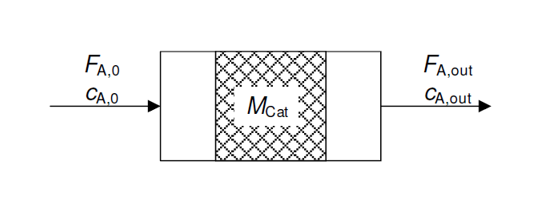
\includegraphics[width=0.6\textwidth]{Graphics/integralreactor.PNG} 
\caption[Schema eines Integralrohrreaktors]{Schema eines Integralrohrreaktor \cite{Skript_2018}}
\label{Integralreactor}
\end{figure}
\noindent
Wobei die Design-Gleichung des Reaktors lautet:

\begin{equation}
\label{eq:design_int}
\frac{M}{F_{HAc,0}}=\int_{0}^{X_{HAc}} \frac{dX_{HAc}}{-r^{'}_{HAc}}
\end{equation}

Um die Reaktionskonstante für die Hinreaktion berechnen zu können muss zunächst das Zeitgesetz (Gleichung \ref{eq:rate-law}) umgeformt werden. Dabei wird die Reaktionskonstante für die Rückreaktion $k_{rück}^'$ durch die Gleichgewichtskonstante $K$ und die Reaktionskonstante für die Hinreaktion $k_{hin}^'$ ausgedrückt.

\begin{equation}
\label{eq:eq-rate-const}
k'_{rück}=\frac{k'_{hin}}{K}
\end{equation}

Die Konzentrationen der einzelnen Spezies können durch den Umsatz und das Verhältnis von EtOH zu HAc durch die Anfangskonzentration der Essigsäure ausgedrückt werden.

\begin{align*}
    c_{HAc} &= c_{HAc, 0} \cdot (1 - X_{HAc})\\
    c_{EtOH} &= c_{HAc, 0} \cdot y \cdot (1 - X_{HAc})\\
    c_{EtAc} &= c_{HAc, 0} \cdot X_{HAc} \\
    c_{H2O} &= c_{HAc, 0} \cdot X_{HAc}
\end{align*}

Somit ergibt sich für das Geschwindigkeitsgesetz folgender Ausdruck:

\begin{align*}
    -r_{HAc}^{'} &= k_{hin}^{'} \cdot c_{HAc} \cdot c_{EtOH} - k_{rück}^{'} \cdot c_{EtAc} \cdot c_{H2O}\\
    -r_{HAc}^{'} &= k_{hin}^{'} \cdot  c_{HAc, 0} \cdot (1 - X_{HAc}) \cdot c_{HAc, 0} \cdot y \cdot (1 - X_{HAc}) \\
    &- \frac{k'_{hin}}{K} \cdot c_{HAc, 0} \cdot X_{HAc} \cdot c_{HAc, 0} \cdot X_{HAc}
\end{align*}

\begin{equation}
\label{eq:rate-law-modified}
        -r_{HAc}^{'} &=  k^{'}_{hin} \cdot c_{HAc,0}^2 \cdot \left((1-X_{HAc})^2 \cdot y - \frac{X_{HAc}^2}{K} \right) 
\end{equation}

Das Verhältnis von Alkohol zu Essigsäure $y$ berechnet sich aus den tatsächlich gemessenen Massenströmen und den daraus berechneten Stoffströmen:

\begin{equation}
    y = \frac{F_{EtOH, 0}}{F_{HAc, 0}}
\end{equation}

\begin{center}
    mit
\end{center}
\begin{equation*}
    F_{A,0} = \frac{\dot{m}_{A,0}}{M_A}
\end{equation*}

Um die Gleichgewichtskonstante für die herrschende Reaktionstemperatur zu berechnen, wird das Van-'t-Hoff'sche Gesetz verwendet. Dazu muss zunächst die Standard-Reaktionsenthalptie aus den Standard-Bildungsenthalpien der einzelnen Reaktanden berechnet werden. Die Enthalpien sind in Tabelle \ref{tab:Bildungsenthalpien} aufgelistet.

\begin{equation}
\Delta H_{R}^0 = \Delta H_{f,prod}^0 - \Delta H_{f,edu}^0
\end{equation}


\begin{table}[H]
	\caption{Bildungsenthalpien der einzelnen Reaktanden}
	\centering
	\begin{tabular}{cccc}
		\toprule 
		Reaktand & $\Delta H^{\circ}_f$ in $\frac{\text{kJ}}{\mole}$ & Quelle & Abweichung \\
		\midrule
		HAc& -483.52 &\cite{Essigsaure_Bildungsentahplie} & ± 0.36 \\
		EtOH& -277.0 &\cite{Ethanol_Bildungsenthalpie} & ± 0.3 \\
		\midrule
		EtAc&  -445.43 &\cite{Ethylacetat_Bildungsenthalpie} & ± 0.84\\
		$\ce{H2O}$& -285.830 & \cite{Wasser_Bildungsenthalpie} & ± 0.040\\
		\bottomrule
	\end{tabular}
	\label{tab:Bildungsenthalpien}
\end{table}


Kirba{\c{s}}lar et al. \cite{kirbacslar2001esterification} haben für diese Reaktion eine Gleichgewichtskonstante von $K_{80} = 4.0$ bei einer Temperatur von 80\,°C ermittelt. Diese Gleichgewichtskonstante wird nun über das Van-'t-Hoff'sche Gesetz auf die Gleichgewichtskonstante bei 60\,°C umgerechnet.

\begin{equation}
K_{60}=K_{80}\cdot\exp\left(-\frac{\Delta H_R^0}{R}\cdot\frac{1}{T_{80}}-\frac{1}{T_{60}}\right)
\end{equation}

Nun wird das veränderte Zeitgesetz aus Gleichung \ref{eq:rate-law-modified} in die Design-Gleichung \ref{eq:design_int} eingesetzt, nach $k'_{hin}$ aufgelöst und integriert:

\begin{align*}
k'_{hin}&=\frac{F_{HAc,0}}{M\cdot c^2_{HAc,0}}\cdot\int_{0}^{X_{HAc}}\frac{1}{(1-X_{HAc})^2\cdot y-\frac{X^2_{HAc}}{K_{60}}}\cdot dX_{HAc}\\
\\
k'_{hin}&=\frac{F_{HAc,0}}{M\cdot c^2_{HAc,0}}\cdot\left\frac{\sqrt{K_{60}} \cdot \tanh^{-1}\left(\frac{K_{60} \cdot y - \frac{1}{2} \cdot \left(X \cdot \left(2 \cdot K_{60} \cdot y - 2 \right) \right)}{\sqrt{K_{60} \cdot y}}\right)}{\sqrt{y}}\right|^{X_{HAc}}_{0}
\end{align*}

Mit $k'_{hin}$ kann über Gleichung \ref{eq:rate-law-modified} die Reaktionsrate $-r_{HAc}^'$ berechnet werden. Über den Zusammenhang von Gleichgewichtskonstante und Reaktionskonstanten (Gleichung \ref{eq:eq-rate-const}) kann die Reaktionskonstante für die Rückreaktion $k'_{rück}$ bestimmt werden.

Die Berechnungen wurden für jeden Umsatz (bzw. jede Probe) durchgeführt, und aus den berechneten Zielgrößen ($-r_{HAc}^'$, $k_{hin}^'$, $k_{rück}^'$) wurde für jede Verweilzeit der Mittelwert mit Standard-Abweichung gebildet.

Die somit erhaltenen Ergebnisse sind in Tabelle \ref{tab:ergebnisseintegral} auf Seite \pageref{tab:ergebnisseintegral} zum leichteren Verständnis mit den Ergebnissen der Differentialmethode dargelegt. 

\section{Differentialmethode}

Die Differentialmethode zur Analyse eines integralen Reaktors, wie zum Beispiel der Rohrreaktor einen darstellt, wird angewandt wenn das Integral zur Lösung der Integralmethode eine Schwierigkeit darstellt \cite{Skript_2018, Levenspiel}. Durch Bilden des Differentials der Designgleichung und Plotten des Umsatzes $X_{HAc}$ gegen die Masse des Katalysators $M$ in kg durch den Molenstrom $F_{HAc}$ in mol$\cdot$s$^{-1}$ kann ein Fit für die Funktion ermittelt werden. Das Differential lässt sich dabei folgendermaßen darstellen, wobei der Molenstrom zum besseren Verständnis nicht mit $N_{HAc}$ wie in Tabelle \ref{tab:Umsatzzusammenfassung} sondern mit $F_{HAc}$ indiziert wird.

\begin{equation}
 d\left(\frac{M}{F_{HAc}}\right) = d\left(\int_{0}^{X_{HAc}} \frac{dX_{HAc}}{-r^{'}_{HAc}}\right)    
\end{equation}
\\
\noindent
Die Reaktionsrate bezogen auf die Masse des Katalysators $-r^{'}_{HAc}$ kann beschrieben werden durch Umformen obiger Gleichung als:

\begin{equation}
\label{raableitung}
    -r^{'}_{HAc} = \frac{dX_{HAc}}{d\left(\frac{M}{F_{HAc}}\right)}
\end{equation}
\\
\noindent
Wird also mit den Messdaten der Plot wie in Abbildung \ref{Differentialanalysis}/Seite \pageref{Differentialanalysis} gebildet und der Fit mit der Matlab-Funktion 'polyfitzero' durch eine quadratische Funktion mit Start im Ursprung ermittelt, kann die Fitfunktion durch folgende Gleichung beschrieben werden ($y = a\cdot x^2 + b\cdot x$):

\begin{equation}
    X_{HAc,fit} = - 1,883 \cdot 10^{-6} \frac{M}{F_{HAc,0}}^2 + 0,002099 \cdot \frac{M}{F_{HAc,0}}
\end{equation}
\\
\noindent
Das Bestimmtheitsmaß des Fits liegt bei $R^2$ = 77,8\,$\%$.
Die Steigung dieser Funktion entspricht der Reaktionsrate $-r_{HAc}^'$, daher wird der Fit einmal nach $M/F_{HAc,0}$ differenziert.

\begin{equation}
-r_{HAc}^{'} = \frac{dX_{HAc,fit}}{d\left(\frac{M}{F_{HAc,0}}\right)} = 2 \cdot (- 1,883 \cdot 10^{-6}) \cdot \frac{M}{F_{HAc,0}} + 0,002099
\end{equation}

In diese Gleichung werden nun die Werte von $M/F_{HAc,0}$ aus Tabelle \ref{tab:Umsatzzusammenfassung2} auf Seite \pageref{tab:Umsatzzusammenfassung2} eingesetzt und so $-r_{HAc}^'$ für die verschiedenen Verweilzeiten berechnet. 

Nun wird das Geschwindigkeitsgesetz aus Kapitel \ref{sec:integral} (Gleichung \ref{eq:rate-law-modified}, Seite \pageref{eq:rate-law-modified}) nach $k_{hin}^'$ umgeformt und die Reaktionskonstante berechnet.

\begin{equation}
            k^{'}_{hin}  &= \frac{-r_{HAc}^{'}} {c_{HAc,0}^2 \cdot \left((1-X_{HAc})^2 \cdot y - \frac{X_{HAc}^2}{K} \right)}
\end{equation}

\newpage
Mit dem Zusammenhang zwischen den Reaktionskonstanten und der Gleichgewichtskonstante (Gleichung \ref{eq:eq-rate-const}) wird abschließend noch die Reaktionskonstante für die Rückreaktion berechnet.

\begin{equation*}
k'_{rück}=\frac{k'_{hin}}{K}
\end{equation*}

Somit werden für jeden Umsatz (bzw. jede gezogene Probe) die Geschwindigkeitskonstanten ermittelt, und die Ergebnisse der einzelnen Zielgrößen für jede Verweilzeit gemittelt.


\begin{figure}[H]
\centering
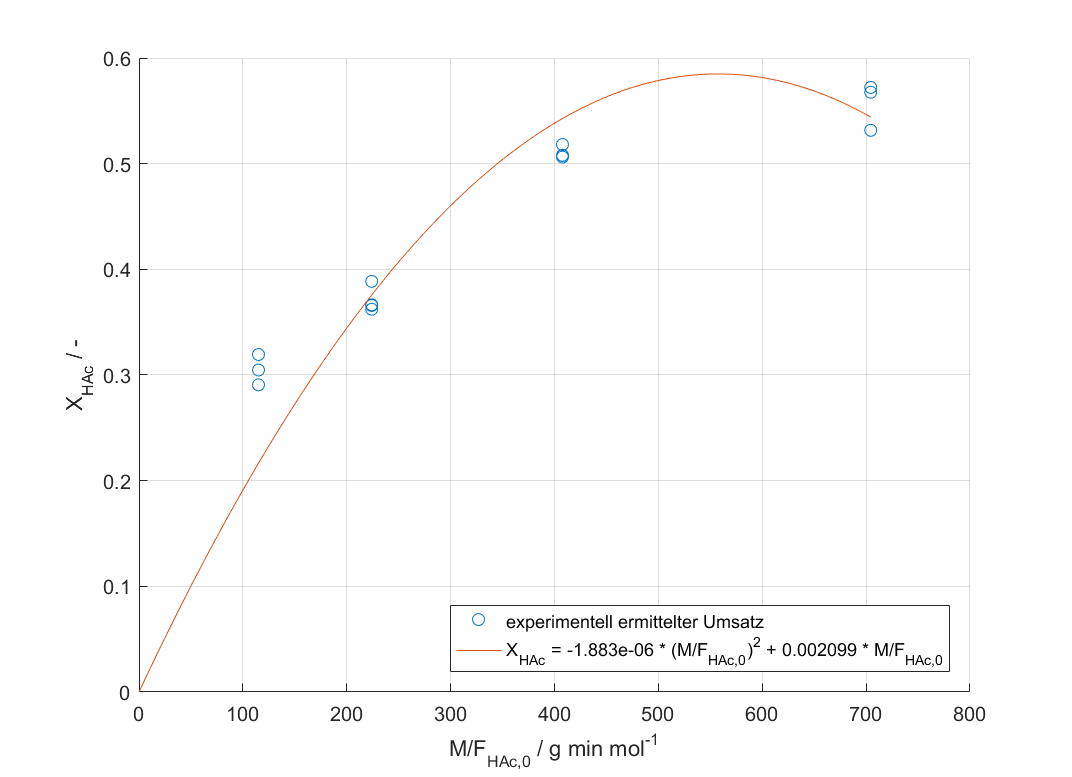
\includegraphics[width=0.8\textwidth]{Graphics/differential_analysis.png} 
\caption{Auswertung der Differentialmethode für die gewählten Verweilzeiten}
\label{Differentialanalysis}
\end{figure}
\noindent
In Abbildung \ref{Differentialanalysis} ist es wichtig zu erwähnen, dass die Datenpunkte von rechts nach links die vier verschiedenen Verweilzeiten abbilden, da durch die Verweilzeit ein anderer Molenstrom $F_{HAc}$ vorhanden ist und somit bei der längsten Verweilzeit der Stoffstrom am geringsten ist und die Werte am weitesten rechts auf der Abszisse liegen. 
\\
\\
Folglich sind die Werte für eine Verweilzeit von $\tau$=15\,min auf dem Teil des Fits befindlich, bei dem eine negative Steigung ermittelt wird und damit physikalisch mit dieser Auswertungsmethode nicht sinnvoll. Die Werte werden daher berechnet aber für weitere Betrachtungen außen vorgelassen. 
\\
\\
Die Ergebnisse der angewandten Differentialmethode sind in Tabelle \ref{tab:ergebnissedifferential} auf Seite \pageref{tab:ergebnissedifferential} zusammengefasst.



\section{Diskussion der gewählten Methoden}

Es könnten auch Berechnungsmethoden mit Differentialreaktoren gewählt werden, da diese aber für geringe Umsätze oder kleine Katalysatormassen gelten \cite{Skript_2018, Levenspiel}. Sie sind  für die erhaltenen experimentellen Ergebnisse nicht anwendbar. Der Vorteil eines Differentialreaktors liegt darin, dass die Reaktionsgeschwindigkeit über den Reaktorverlauf konstant bleibt, da sich die Konzentration nicht bzw. nur minimalst ändert. Daher kann die Reaktionsgeschwindigkeit in der Design-Gleichung vor das Integral gezogen werden, was zu einer erheblich einfacheren Berechnung führt.
\\
\\
Mit den berechneten Ergebnissen der beiden Methoden (siehe folgende Tabellen \ref{tab:ergebnisseintegral} und \ref{tab:ergebnissedifferential}) lassen sich diverse Vergleiche anstellen.

% Table generated by Excel2LaTeX from sheet 'Tabelle1'
\begin{table}[htbp]
  \centering
  \caption{Ergebnisse der Integralmethode}
    \begin{tabular}{r|rcr|rcr|rcr}
    \toprule
    \multicolumn{1}{l|}{$\tau_{real}$ in min}& \multicolumn{3}{c|}{$k'_{integral, hin}$ in $\frac{\text{g}}{\text{mol}\cdot\text{min}}$}  & \multicolumn{3}{c|}{$k'_{integral,rück}$ in $\frac{\text{g}}{\text{mol}\cdot\text{min}}$}  & \multicolumn{3}{c}{$r'_{integral}$ in $\frac{\text{mol}}{\text{g}\cdot\text{min}}$} \\
    \midrule
    14,93 & 26,521 & \multirow{4}[1]{*}{$\pm$} & 2,748 & 7,601 & \multirow{4}[1]{*}{$\pm$} & 0,788 & 0,00029 & \multirow{4}[1]{*}{$\pm$} & 0,00001 \\
    9,57  & 34,996 &       & 0,895 & 10,029 &       & 1,365 & 0,00053 &       & 0,00000 \\
    5,01  & 35,225 &       & 1,926 & 10,095 &       & 1,299 & 0,00100 &       & 0,00001 \\
    2,61  & 50,222 &       & 3,473 & 14,393 &       & 0,301 & 0,00180 &       & 0,00004\\
    \bottomrule
    \end{tabular}%
  \label{tab:ergebnisseintegral}%
\end{table}%
\noindent
Vergleicht man die Reaktionsgeschwindigkeitskonstanten für die Hin- und Rückreaktion aus der Integralmethode, erkennt man dass tendenziell die Hinreaktion schneller abläuft und damit bei gleicher Verweilzeit das Gleichgewicht auf der Seite der Produkte Ethylacetat und Wasser liegen wird. Mit dem allgemeinen Geschwindigkeitsgesetz 

\begin{equation}
 \label{geschwindigkeitsgesetz}
 -r^{'}_{HAc} = k^{'}_{hin} \cdot c_{HAc} \cdot c_{EtOH} - k^{'}_{rück} \cdot c_{EtAc} \cdot c_{H_2O}
\end{equation}
\\
\noindent
kann damit die Reaktionsrate $-r^{'}$ bei den pro Versuch ermittelten Konzentrationen ermittelt werden. Es ist ersichtlich, dass die Abweichung, als Standardabweichung gebildet, für die kürzeste Verweilzeit von $\tau$ =  2,61\,min für die Reaktionsrate  $-r^{'}_{HAc}$ am größten ist. Dies ist höchstwahrscheinlich auf die turbulente Strömung durch den großen Volumenstrom und die damit einhergehenden Strömungs-Nichtidealitäten und Rückvermischungen zurückzuführen. Das Maximum der Abweichungen in der Integralmethode liegt auch bei den Reaktionsgeschwindigkeitskonstanten bei der minimalen Verweilzeit. 
\\
\\
Bei Betrachtung der Differentialmethode fällt als erstes der negative Wert für die Reaktionsrate bei der längsten Verweilzeit auf. Dies ist bereits in Abschnitt 4.4 erklärt, da die Umsätze für diese Verweilzeit zu gering sind und daher der Fit eine negative Steigung aufweist. Die Reaktionsrate kann nicht mit Abweichung angegeben werden, da die Steigung bereits aus dem Fit ermittelt wird welcher den Mittelwert der Datenpunkte heranzieht. Als Folge der negativen Reaktionsrate ergeben sich negative Reaktionsgeschwindigkeitskonstanten, darum werden diese Werte für weitere Betrachtungen verworfen und auf die zu geringe Einlaufzeit des Reaktors zum stationären Zustand zurückgeführt. Wie auch bei der Integralmethode ist die Hin-Reaktion tendenziell um einiges schneller als die Rückreaktion. Die Abweichung der Reaktionsgeschwindigkeitskonstanten wird aus der Reaktionsrate mit Umsätzen und Konzentrationen der anderen Verweilzeiten gebildet. 

% Table generated by Excel2LaTeX from sheet 'Tabelle1'
\begin{table}[htbp]
  \centering
  \caption{Ergebnisse der Differentialmethode}
    \begin{tabular}{c|ccc|ccc|c}
    \toprule
    \multicolumn{1}{c|}{$\tau_{real}$ in min} & \multicolumn{3}{c|}{$k'_{differential, hin}$ in $\frac{\text{g}}{\text{mol}\cdot\text{min}}$} & \multicolumn{3}{c|}{$k'_{differential, rück}$ in $\frac{\text{g}}{\text{mol}\cdot\text{min}}$} & \multicolumn{1}{c}{$r'_{differential}$ in $\frac{\text{mol}}{\text{g}\cdot\text{min}}$} \\
    \midrule
    14,93 & -39,756 & \multirow{4}[1]{*}{$\pm$} & 4,053 & -1,653 & \multirow{4}[1]{*}{$\pm$} & 0,169 & -0,00055 \\
    9,57  & 30,900 &       & 0,742 & 1,285 &       & 0,031 & 0,00056 \\
    5,01  & 41,993 &       & 1,687 & 1,747 &       & 0,070 & 0,00126 \\
    2,61  & 45,124 &       & 1,893 & 1,877 &       & 0,079 & 0,00167 \\
    \bottomrule
    \end{tabular}%
  \label{tab:ergebnissedifferential}%
\end{table}%
\noindent
Im direkten Vergleich der Integral- und Differentialmethode wird ersichtlich, dass die Integralmethode generell genauer ist, da kein Fit benötigt wird und somit keine Abweichung von ca. 30\,$\%$ wie bei der Differentialmethode vorhanden sein kann. Der Vergleich mit anderen experimentellen Werten ist im nächsten Kapitel ersichtlich.

\section{Vergleich der Kinetik}

Zeki et al. \cite{zeki2018kinetic} haben in ihrer Arbeit \glqq Kinetic Study of Esterification Reaction\grqq\;die Kinetik der Veresterungsreaktion von HAc und EtOH mit Schwefelsäure als Katalysator untersucht. Die Experimente wurden isotherm zwischen 50 und 60\,°C in einem 500\,ml Batchreaktor durchgeführt. Die Auswertungen der Arbeit zeigen, dass eine Reaktionsordnung 2-ter Ordnung angenommen werden kann. Reaktionsumsätze von 80\,\% wurden bei 60°C bei einem Molverhältnis (EtOH/HAc) von 10 erreicht. Zusätzlich wird gezeigt, dass längere Verweilzeiten einen höheren Umsatz ergeben, was bei den durchgeführten Versuchen ebenfalls gezeigt werden kann. Bei den durchgeführten Experimenten werden Umsätze von 57\,\% bei einer effektiven Verweilzeit von 14,93 min erreicht, jedoch wird in dieser Arbeit ein anderer Katalysator und ein Molverhältnis (EtOH/HAc) von 2:1 verwendet.

Kirba{\c{s}}lar et al. \cite{kirbacslar2001esterification} haben in ihrer Arbeit \glqq Esterication of Acetic Acid with Ethanol Catalysed by an Acidic Ion-Exchange Resin\grqq\;die Veresterung von Essigsäure mit Ethylalkohol, katalysiert durch $\text{Amberlyst}^\text{\textregistered}$15 in einem Batch-Reaktor bei Temperaturen zwischen 323 und 353\,K bei verschiedenen Ausgangsbedingungen durchgeführt und untersucht. Im Zuge ihrer Arbeit testeten sie die Wiederverwendbarkeit des Katalysators. Dabei wurde der gleiche Versuch dreimal wiederholt und mit einander verglichen. Eine Abweichung des Reaktionsumsatzes von 5\,\% wurde festgestellt. Es wurde eine maximale Essigsäureumsetzung von 75\,\% mit einem Molverhältnis (EtOH/HAc) von 2 bei 353\,K und 5,4\,g/100\,g HAc erreicht.
\\
\\
Die erhaltenen Umsätze aus den Konzentrationen können bei verschiedenen Verweilzeiten mit den gewählten Methoden der Differential- und Integralmethode zur Ermittlung der Reaktionsgeschwindigkeitskonstante herangezogen werden.
\\
\\
%In der Literatur werden dabei z.B. bei heterogen katalysierter Reaktion mit $\text{Amberlyst}^\text{\textregistered}$15 folgende Werte für den präexponentiellen Faktor für die Hin- (Index 1) und Rückreaktion (Index 2) gestellt. 
%
%\begin{table}[H]
%	\caption{Vergleich der Kinetik}
%	\centering
%	\begin{tabular}{cccc}
%		\toprule 
%		Quelle & Referenz $T$ in K & $k_1^0$ & $k_2^0$  \\
%		\midrule
%		\cite{calvar2007esterification} & 303-353\,K &161,29\,$\frac{\text{mol}}{\text{s}\cdot\text{kg}}$ & 8,34\,$\frac{\text{mol}}{\text{s}\cdot\text{kg}}$ \\
%		\cite{calvar2007esterification} & 303-353\,K & 2,811\,$\frac{\text{mol}}{\text{s}\cdot\text{kg}}$ & 0,051\,$\frac{\text{mol}}{\text{s}\cdot\text{kg}}$ \\
%		\bottomrule
%	\end{tabular}
%	\label{tab:KinetikVergleich}
%\end{table}
%\noindent
%Die signifikante Abweichung der Stoßfaktoren im Arrhenius-Gesetz aus \cite{calvar2007esterification} für die Hin- und Rückreaktion kann auf die unterschiedliche Berechnung der Aktivitäten zur Bestimmung des Zeitgesetzes zurückgeführt werden. Als Methoden wurden von den Autoren ASOG (Analytical Solution of Groups) und UNIFAC (Universal Quasichemical Functional Group Activity Coefficients) verwendet, wobei ASOG für den Aktivitätskoeffizienten der Essigsäure immer Werte kleiner 1  und UNIFAC Werte größer 1 ausgibt. 
%\\
%\\
%Mithilfe der gegebenen Stoßfaktoren könnte man bei bekannter Aktivierungsenergie und der vorhandenen Temperatur von 60\,°C eine Reaktionsgeschwindigkeitskonstante für Hin- und Rückreaktion bestimmen. Auf weitere Vergleiche der Reaktionsgeschwindigkeitskonstanten wird verzichtet, da in den angegebenen Werken bzw. Veröffentlichungen wenige Werte dafür angegeben werden. Zudem würde sich ein direkter Vergleich als schwierig erweisen, da die Reaktionsgeschwindigkeitskonstanten stark vom experimentellen Aufbau abhängig sind.
%\\
%\\
Laut \cite{beula2015kinetics} ist die Esterifikation eine langsame und hoch reversible Reaktion, welche durch vier Möglichkeiten zugunsten der Produkte beeinflusst werden kann: Zuführen des Alkohols im Überschuss, Verwenden eines hygroskopischen Reagenz, Entfernen von Wasser und Verwendung eines Katalysators. Aus diesem Grund kann als Katalysator auch eine Säure für eine homogene Katalyse verwendet werden. In der Arbeit werden bei einer Reaktionstemperatur von 60\,°C im Batch-Versuch bei einem Molverhältnis von 2:1 EtOH zu HAc folgende Reaktionsgeschwindigkeitskonstanten erhalten:


\begin{table}[H]
	\caption{Geschwindigkeitskonstanten nach Beula (2015)}
	\centering
	\begin{tabular}{cccc}
		\toprule 
		Quelle & Referenz $T$ in K & $k_{hin}$ & $k_{rück}$  \\
		\midrule
		\cite{beula2015kinetics} & 60 & 22,35\,$\frac{\text{cm}^3}{\text{mol}\cdot \text{min}}$ & 22,35\,$\frac{\text{cm}^3}{\text{mol}\cdot \text{min}}$ \\
		\bottomrule
	\end{tabular}
	\label{tab:KinetikVergleich1}
\end{table}
\noindent
Die Werte für die Reaktionsgeschwindigkeitskonstante weichen von den in dieser Arbeit erhaltenen unter Berücksichtigung der Einheiten stark ab (berücksichtigt wird mittels der angenommenen Dichte des Gemisches von 1\,g $\cdot$ cm$^3$), was auf diverse Gründe zurückgeführt werden kann. Erstens ist die Katalyse homogen und nicht heterogen bzw. ist die Menge des Katalysators nicht direkt vergleichbar, zweitens wird ein Batch-Reaktor verwendet und drittens sind die Verweilzeiten nicht mit einem Rohrreaktor zu vergleichen. Grundsätzlich sind die Werte im Sinne der Zehnerpotenz ähnlich. Bei Berücksichtigung der aufgelisteten Gründe kann daher eine positive Evaluierung ausfallen.


% Laut IndianChemicalEngineer ist die Esterifikation eine langsame und hoch reversible Reaktion, welche durch vier Möglichkeiten zugunsten der Produkte beeinflusst werden kann: Zuführen des Alkohols im Überschuss, Verwenden eines hygroskopischen Reagenz, Entfernen von Wasser und Verwendung eines Katalysators. Aus diesem Grund kann als Katalysator auch eine Säure für eine homogene Katalyse verwendet werden. 

% In der Literatur werden die Umsätze oft auf den Gleichgewichtsumsatz bezogen bzw. die experimentelle Durchführung derart gestaltet, dass dieser Umsatz erreicht wird. Aus diesem Grunde können Umsätze nur schwer mit der Literatur verglichen werden.



\section{Mögliche Fehlerquellen und Verbesserungsmöglichkeiten}

Vor dem Beginn der Versuche wird der Reaktor durch gezielte Druckstöße entlüftet um vorhandene Gasblasen darin zu entfernen. Im Verlauf der Versuche konnten jedoch immer wieder Gasblasen im Reaktor festgestellt werden. Diese beeinflussen durch die Querschnittsveränderung der Flüssigphase und deren Aufsteigen im Reaktor  die Strömung maßgeblich. Die Querschnittsveränderung der Flüssigphase erhöht die Strömungsgeschwindigkeit punktuell und verursacht in Folge axiale Rückvermischungen. Ebenso tragen aufsteigende Gasblasen zu einer axialen Vermischung der Komponenten bei.
Eine weitere Quelle axialer Vermischungen ist die nicht kontinuierliche Arbeitsweise der Peristaltikpumpen, welche durch die impulsweise Zudosierung Druckstöße generiert.

Mit zunehmendem Durchsatz verteilt sich der Katalysator zunehmend über das gesamte Reaktorvolumen. Dadurch ist nicht mehr der gesamte Rohrquerschnitt mit Katalysator gefüllt sondern in etwa die Hälfte davon. Das hat zur Folge, dass sich die Strömung bevorzugt in der oberen Hälfte des Rohrquerschnitts ausprägt und die Strömung durch die Zwischenräume der Katalysatorschüttung verringert wird. Der intensive Phasenkontakt einer Strömung durch eine dichte Kugelpackung ist somit nicht mehr gegeben, sondern deutlich verringert.
Dieser Nichtidealität könnte durch eine fixierte Feststoffpackung engegengewirkt werden. Jedoch ist zu beachten, dass eingetragene oder entstehende Gasblasen dadurch deutlich am Wiederaustreten gehindert werden.

Wie bereits in der Durchführung erwähnt, wird auf eine möglichst rasche Analyse nach der Probenahme geachtet und die Proben in diesem Zeitraum gekühlt um den Verlust der flüchtigen Komponenten (EtOH, EtAc) zu minimieren und eine weitere Reaktion zu unterbinden. Dieser Verlust kann jedoch - ebenso wie eine weitere Reaktion - aufgrund von örtlichen Unterschieden der Probenahme und Auswertung nicht zur Gänze ausgeschlossen werden.

Eine weitere mögliche Fehlerquelle ist die Temperatur der Komponenten am Reaktor Eintritt. Zwar werden die Vorlagen vor den Versuchen vorgewärmt und ein Wärmetauscher vor dem Reaktor verwendet, jedoch ist zu beachten, dass die Temperatur der Vorlagen mit der Zeit abnehmen und mit steigendem Durchsatz die verhältnismäßig kleinen Wärmetauscher möglicherweise nicht mehr die nötige Heizleistung bereitstellen können. Dadurch ist die konstante Reaktortemperatur von 60\,$\text{°C}$ - vor allem bei den Versuchsreihen mit höheren Durchsätzen - nicht garantiert. Weiter wurde die Dichte von Ethanol und Essigsäure bei 20\,°C bestimmt. Mit diesen Ergebnissen wurde dann die Umdrehungszahl der Pumpe bestimmt, jedoch wurden die Versuche bei 60\,°C durchgeführt. Die höhere Temperatur der Flüssigkeiten bewirkt ein größeres Volumen und somit auch einen verfälschten Volumenstrom.

Um einen stationären Betrieb zu erreichen werden die neuen Volumenströme die 3-fache theoretische Verweilzeit vor der Probenahme  zudosiert. Trotzdem sind Abweichungen in den Proben der ersten Versuchsreihe festzustellen, welche auf eine zu kurze Einlaufzeit schließen lassen. Dies könnte auf eine von der gegebenen abweichende Zusammensetzung im Reaktor zurückzuführen sein, welche sich mit der Zeit der gewünschten Zusammensetzung mit fortlaufender Versuchszeit annähert. Das spiegelt auch die Ergebnisse der ersten Versuchsreihe wieder, die einen steigenden Umsatz mit fortschreitender Zeit aufweist. Folglich ist der stationäre Zustand, welcher bei der Verweilzeit von 15\,min anzustreben ist, nicht erreicht, es wäre also eine längere Einlaufzeit zum stationären Zustand des Reaktors abzuwarten.
\\
\\
Bei der Durchführung des Versuches ist der Zustand des Katalysators zu beachten. Einen unerwünschten Zustand des Katalysators stellen zum Beispiel Fouling, Vergiftung oder Sintern dar \cite{mortimer2007chemie}. Fouling ist als mechanische Anlagerungen am Katalysator zu verstehen. Voraussetzung für solch eine Anlagerung ist die Größe der angelagerten Partikel. Diese müssen kleiner als der Porendurchmesser des Katalysators sein. Die Partikel können aus jeglichen Stoffen bestehen, welche sich im System befinden und keine chemische Bindung mit dem Katalysator eingehen. Die Vergiftung im Gegenzug entsteht bei der chemischen Bindung von Stoffen mit dem Katalysator. Diese Stoffe sind zum Beispiel Schwermetalle, Schwefel oder Halogene. Die Anlagerungen vermindern die aktive Oberfläche der Katalysatoren in den Poren. Dies führt zu einer Verminderung der katalytischen Wirkung und der Geschwindigkeitskonstante. Für das Sintern des Katalysators ist eine hohe Temperatur notwendig. Der Versuch wird mit 60\,°C und bei Umgebungsdruck gefahren, weshalb für Sintern keine Gefahr besteht. Die maximale Arbeitstemperatur von $\text{Amberlyst}^\text{\textregistered}$15 ist laut Hersteller 120\,°C \cite{Amberlyst_Stoffdaten}.\newline

Im Versuchsaufbau fungiert der Mischer mit den Raschigringen als statischer Mischer. Statische Mischer haben je nach Ausführung und Handhabung einen begrenzten Mischungsgrad. Sie sind zum Beispiel nicht für lange Verweilzeiten geeignet \cite{zogg1993einfuhrung}. Eine weitere Möglichkeit der Mischung wäre daher das Voranschalten eines Durchlauf-Rührmischers mit mehreren Rührwerken (kleine Verweilzeiten) oder mehrstufige Rührkolonnen (große Verweilzeiten) vor dem Strömungsrohr \cite{zogg1993einfuhrung}. Um den Versuch nicht zu verfälschen, müssten diese Ausführungen ausreichend gekühlt werden, um die Reaktion anzuhalten, denn wichtig ist die Analyse des Umsatzes \textbf{nur} im Strömungsrohr. Vorraussetzung für die Auswertung ist daher eine homogen-verteilte Lösung, bei der die Reaktion beim Eintritt ins Strömungsrohr noch nicht begonnen hat.

\chapter{Zusammenfassung und Ausblick}
Abschließend werden die Ergebnisse respektive auf die einzelnen Unterpunkte geschildert und interpretiert. \newline

Zu Beginn wurde der Umsatz der Reaktion bei verschiedenen Verweilzeiten bestimmt. Während dieser Berechnung ist die Abweichung der idealen eingestellten zur real gemessenen Verweilzeit ersichtlich. Die Abweichungen befinden sich jedoch  im Toleranzbereich und stellen repräsentative Werte dar. Die Abweichungen werden durch das Auf- bzw. Abrunden der Umdrehungszahleinstellung der Pumpe generiert. \newline
Die Versuche sollten mit einem Molverhältnis von EtOH zu HAc von 2 durchgeführt werden. Mit dem gemessenen realen Massenstrom konnte so die tatsächlichen Molenströme ermittelt werden, welche in Tabelle \ref{tab:Umsatzzusammenfassung} tabelliert sind. Weiters ermittelt sich im Laufe der Berechnungen ein Molenbruch, der im Durchschnitt für alle Verweilzeiten um die 1,75 liegt. Das eingestellte Molverhältnis wurde demnach leicht unterschritten. Dies ist ebenfalls auf die Einstellungen der Pumpe zurückzuführen. \newline
In Tabelle \ref{tab:Umsatzzusammenfassung2} ist der Umsatz ersichtlich. Es zeichnet sich klar ab, dass bei höheren Verweilzeiten bessere Umsätze erzielt werden können, was den Erwartungen entspricht. Dies liegt vor allem auch am Verhältnis zwischen Katalysatormasse und Molenstrom Essigsäure. Bei kleinen Verweilzeiten ergeben sich kleine Verhältnisse, was ebenfalls durch das erhaltene Ergebnis unterstrichen wird.\newline

Die Reaktionsordnung wird der Literatur entnommen. Zur eigentlichen Bestimmung wird die Gleichung der Reaktionsrate herangezogen. Da dies nicht die primäre Aufgabe dieser Laborübung ist, kann auf experimentelle Werte aus Literatur verwiesen werden. In diversen wissenschaftlichen Schriften wird die Essigsäureveresterung mit einer reversiblen Reaktion \textbf{zweiter Ordnung} beschrieben.\newline

Zur Datenanalyse der Reaktion wird sowohl die Integral- als auch die Differentialmethode verwendet. Der Reaktor wurde als Integralreaktor betrachtet. Über die Integralmethode lässt sich die Geschwindigkeitskonstante und schließlich die Reaktionsrate berechnen (über Konzentration und Reaktionsordnung). Die Differentialmethode liefert mittels eines grafischen Ansatzes die Reaktionsrate. Sie ist die gemittelte Steigung an den Messpunkten einer Regressionsfunktion mit $\nicefrac{M_{cat}}{F_{HAc,0}}$ als Abszisse und $X_{HAc}$ als Ordinate.\newline
Die Hinreaktion der behandelten Esterifikation läuft in der Regel schneller ab als die Rückreaktion. Das bedeutet es werden mehr Produkte als Edukte gebildet. Durch die stark laminare Strömung und die dadurch entstehende Rückvermischung bei $\tau=15\,\text{min}$ zeigt sich die größte Abweichung bei der Berechnung der Reaktionsrate und der Geschwindigkeitskonstante bei Verwendung der Integralmethode. \newline
Die Differentialmethode gilt allgemein als ungenauer, da der grafische Ansatz durch die Regression an Genauigkeit verliert. Im direkten Vergleich zeigt sich, dass die Abweichung zur Integralmethode bis zu 30\,\% beträgt. 

Die Abweichungen in den Umsätzen können wie bereits erwähnt bei der längsten Verweilzeit über den noch nicht erreichten stationären Zustand und bei den geringeren Verweilzeiten über Strömungs-Nichtidealitäten erklärt werden. Hinsichtlich den starken Schwankungen der Reaktionsgeschwindigkeitskonstanten aus der Integralmethode lassen sich die experimentellen Fehler durch Verdampfen der flüchtigen Komponenten und weiteres Reagieren durch nicht ausreichendes Kühlen der Reaktanden anführen. Die Ergebnisse der Differentialmethode sind aufgrund der Regression der quadratischen Funktion mit Vorsicht zu genießen, da ein negativer Wert ermittelt werden kann und daher ein Fehler in den Messdaten, welche zum Generieren des Fits herangezogen werden, festgestellt werden kann.

Hinsichtlich der Fehlerquellen wird an dieser Stelle auf Sektion 4.7 verwiesen, da die Fehlerquellen Hand in Hand mit den Verbesserungsmöglichkeiten gehen.

Die berechneten Werte für die Geschwindigkeitskonstanten sind bei erster Analyse durch eine hohe Abweichung mit Literaturwerten aufgefallen. Bei Berücksichtigung der zuvor genannten Gründe wie zum Beispiel Menge und Art des Katalysators sind die berechneten Werte als repräsetnativ einzustufen. 

Ausblickend könnte der Versuch weitergeführt werden. Eine Möglichkeit für die Auswertung wäre der Vergleich der Kinetik aus dem Experiment mit der Literatur, jedoch für die unkatalysierte Reaktion. Dafür müsste der Versuch unkatalysiert durchgeführt werden. Dabei müsste der Diffusionskoeffizient der Flüssigkeiten Essigsäure und Ethanol bestimmt (wobei $D$ für Flüssigkeiten in der Größenordnung von $10^{-9}$\,$\text{m}^2/$s liegen \cite{mortimer2007chemie}) werden und damit die tatsächliche Reaktionsgeschwindigkeitskonstante aus den berechneten Werten kalkuliert werden, indem folgende Gleichung manipuliert wird \cite{Skript_2018}:

\begin{equation}
 k'_{kat} = \sqrt{\frac{2}{n +1} \cdot \frac{k_{unkat} \cdot D_{eff}}{L^2}}
\end{equation}
\noindent
Die Anwendung der charakteristischen Länge $L$ und der Reaktionsordnung wäre in diesem Fall $L$ für sphärische Partikel und Reaktionsordnung von $n$=2. Dies ist jedoch nicht das primäre Ziel dieser Laborübung und daher wird bei der Auswertung auf zukünftige Arbeiten verwiesen. 

\newpage
\pagenumbering{arabic}

\newpage
 \pagenumbering{Roman}
\setcounter{page}{2}

\newpage
\listoffigures

\newpage
\listoftables


\newpage

%\bibliography{quellen} 
%\bibliographystyle{ieeetr}
%\addcontentsline{toc}{chapter}{Literaturverzeichnis}
\bibliographystyle{unsrtdin}
\addcontentsline{toc}{chapter}{Literaturverzeichnis} 
\bibliography{Literatur_CRT_2_2}
\printbibliography








%\appendix
%\chapter*{Anhang}
%\addcontentsline{toc}{chapter}{Anhang}


\end{document}
